%************************************************
\section{Scenario 1: WarmupTask} % (fold)
\label{sec:eval_warmup_scenario}
%************************************************
This first scenario is meant to make you familiar with the simulator's concepts and interactions. The environment is made up by two tables; the first table has two items on it: a pen and a small statue. The other table is empty. All entities in this scenario can be interacted with. A screenshot of the running simulation is depicted in Figure \ref{fig:eval_warump}.\\

\begin{figure}[H]
	\centering
	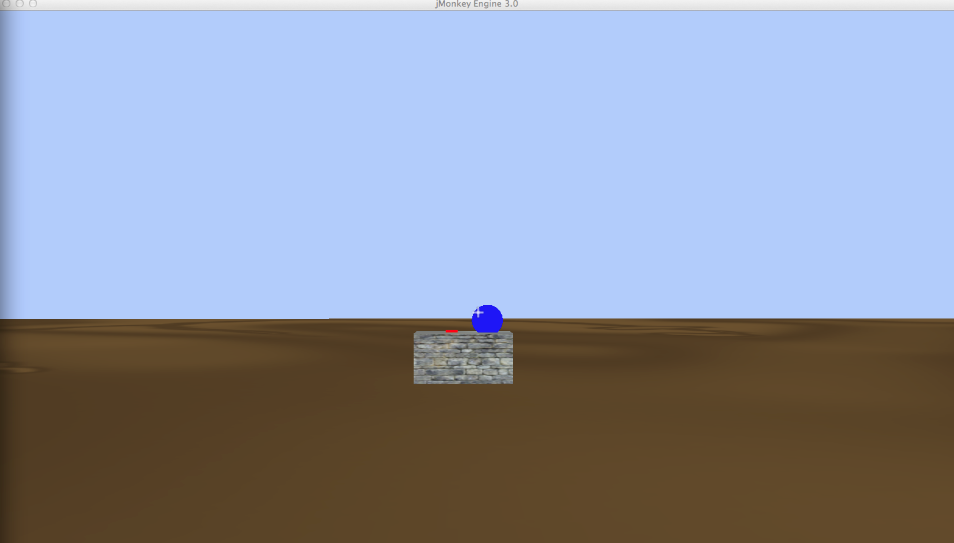
\includegraphics[width=0.8\linewidth]{gfx/Chapter_EvaluationScenarios/prototype1}
	\caption{Sceenshot of the running Warm-up simulation}
	\label{fig:eval_warump}
\end{figure}

Your task is to walk around and interact with the environment while observing the SSM spaces in the ContextClient. N.B.: The client is automatically refreshed every second. As part of the actions you carry out, please try out the followings:
\begin{enumerate}
	\item Move far away from the first table (facing the table), until in the perception space contains only Table1 (it might contain Table2 as well if it's in your visual range). Slowly move towards Table1. At certain distances the PerceptionSpace, RecognizableSet and ExaminableSet will be populated.
	\item Try interacting with the pen while it IS NOT part of the ActionSpace. You are informed that the agent is too far.
	\item Try interacting with the pen while it IS part of the ActionSpace. The pen gets picked up.
	\item Move with the pen towards Table2. While Table2 IS NOT in the ActionSpace, try to interact with it. You are informed that the agent is too far.
	\item While Table2 IS in the ActionSpace and with the pen picked up, try to interact with the table. Table2 is a surfaces and the pen can be placed onto it.
	\item While not holding anything in your hands and while Table2 IS in the ActionSpace, try to it up. Table2 is too heavy for the agent carry.
	\item Move towards the Statue until it's in the ActionSpace and try to interact with it. Interacting with the Statue requires a different implementation than the standard piking up object which is not implemented in this iteration.
	\item Pick up the pen. With the pen picked up and the statue in the ActionSpace, try to interact with the Statue. You can't, because Statue is not a surface. Future releases will handled this more complex scenario as well.
\end{enumerate}

When you arrive to this point, you have successfully performed the WarmUp Task.
% section eval_warmup_scenario (end)